\documentclass{article}

\usepackage{header}
\usetikzlibrary{patterns}
\usetikzlibrary{calc}

\title{Rapport de la r\'eunion sur les paradigmes de simulations temps r\'eel}
\author{C.MASCART}

\begin{document}
	\maketitle
	\section*{RTDEVS actuel}
		\begin{figure}[H]
			\begin{center}
				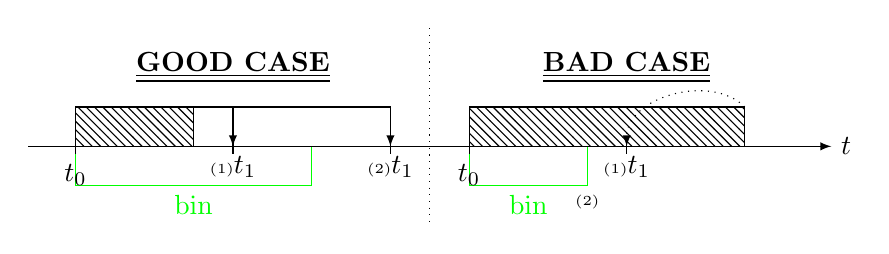
\begin{tikzpicture}
					% Coordinates of the first and second part of the figure
					\coordinate (O1) at (0.5,0);
					\coordinate (O2) at (5.5,0);

					% Put in first so that it is recovered by the time line
					\draw[color=green] ($(O1)+(0,0)$) rectangle ($(O1)+(3,-0.5)$) node [midway, below=0.25cm] {{\color{green}bin}};
					\draw[color=green] ($(O2)+(0,0)$) rectangle ($(O2)+(1.5,-0.5)$) node [midway, below=0.25cm] {{\color{green}bin}};
					\node[below] (bcgr) at ($(O2)+(1.5,-0.5)$) {\tiny(2)};

					\draw[-latex] (-0.1, 0) -- (10.1, 0) node [right] {$t$};
					\draw[dotted] (5, 1.5) -- (5, -1);
					\node (gc) at (2.5, 1) {\underline{\underline{\textbf{GOOD CASE}}}};
					\node (bc) at (7.5, 1) {\underline{\underline{\textbf{BAD CASE}}}};

					\draw ($(O1)+(0,0.1)$) -- ($(O1)+(0,-0.1)$) node [left, below] {$t_0$};
					\draw ($(O1)+(2,0.1)$) -- ($(O1)+(2,-0.1)$) node [midway, below] (gct11) {{\tiny(1)}$t_1$};
					\draw ($(O1)+(4,0.1)$) -- ($(O1)+(4,-0.1)$) node [midway, below] (gct12) {{\tiny(2)}$t_1$};
					\draw[pattern=north west lines] (O1) rectangle ($(O1)+(1.5,0.5)$) node (gcr) {};
					\draw[-latex] (gcr.base) -| (gct11);
					\draw[-latex] (gcr.base) -| (gct12);

					\draw ($(O2)+(0,0.1)$) -- ($(O2)+(0,-0.1)$) node [left, below] {$t_0$};
					\draw ($(O2)+(2,0.1)$) -- ($(O2)+(2,-0.1)$) node [midway, below] (gct11) {{\tiny(1)}$t_1$};
					\draw[pattern=north west lines] (O2) rectangle ($(O2)+(3.5,0.5)$) node (gcr) {};
					\draw[-latex, dotted] (gcr.base) to[out=135, in=90] (gct11);
				\end{tikzpicture}
			\end{center}
			\caption{Good case execution vs. Bad case execution. The hatched area corresponds to the execution time of the tasks at $t_0$.}\label{fig:gcbc}
		\end{figure}
		On \'ex\'ecute tous les \'ev\'enements \`a $t_0$ temps actuel (physique et de simulation). Tant qu'il reste des \'ev\'enements \`a ex\'ecuter \`a $t_0$ (potentiellement ordonnanc\'es \`a $t_0$, par un $\mathrm{holdin}("...", 0)\implies\sigma=0$) \`a $t_0$ on continue, sauf si le temps r'eel d\'erive au-del\`a de la limite impos\'ee par la {\color{green}bin} (c.f. on fig~\ref{fig:gcbc} good cases and bad case~(1)). On regarde ensuite que les \'ev\'enements futurs se passeront \`a un temps physique futur (c.f. on fig~\ref{fig:gcbc} bad case~(2)). Si tel est le cas on \'eteint la simulation jusqu'\`a ce que le temps physique atteigne le TNext de simulation.\\
		On garde ainsi une approche purement "\'ev\'enements discrets", avec l'approximation que les \'ev\'enements \`a $t_0$ se passeront effectivement \`a $t_0$ et pas \`a $t_0+\delta t$, le $\delta t$ provenant du temps d'ex\'ecution des fonctions de transitions (et de toute la machinerie DEVS).\\
		La "granule" (que j'ai ici renom\'e {\color{green}bin} pour des raisons \'evidentes d'hygi\`ene nomenclatique) joue ici le r\^ole d'une borne sup\'erieure de temps.

	\section*{Temps r\'eel \emph{\`a la} SpinNaker}
		\begin{figure}[H]
			\begin{center}
				\begin{tikzpicture}
					\draw[-latex] (-0.1, 0) -- (10.5, 0) node [right] {$t$};
					\foreach \x in {1,2,3,4,5,6} {
						\draw ({2*(\x-1)},0.1) -- ({2*(\x-1)},-0.1) node (t\x) [below] {\x};
					}
					\foreach \x in {0.5, 0.75, 1.25, 7.25} {
						\draw[*-] (\x, 1) -- (\x, 0);
					}
					\draw[latex-latex] (t2) -- (t3) node [midway, below] {granule = $\Delta t$};
				\end{tikzpicture}
			\end{center}
			\caption{Mailage de la ligne de temps et r\'epartition des \'ev\'enements sur icelle.}\label{fig:rtsn}
		\end{figure}
		On a ici un maillage strict de la ligne de temps avec un pas de temps constant $\Delta t$, que l'on appellera la granule. Cette granule est en fait plus ou moins artificielle, elle est reli\'ee \`a la fr\'equence d'\'echantillonage du temps pour un OS (la gestion des \'ev\'enements n\'ec\'essitant souvent d'attendre pendant certaines p\'eriodes de temps), ou les ticks d'horloge du processeur.


\end{document}